%\documentclass[14pt]{report} 
\documentclass[14pt]{../sty/NSLReport} % Базовый стиль - поправленный стандартный report, они взаимозаменяемы
%\documentclass[14pt, twoside]{../sty/NSLReport} % Включает режим двусторонний режим, неудобно для просмотра pdf

\RequirePackage{../sty/NSLExtra} % Расширение над NSLReport, включая longtable, caption, biblatex и прочие must have пакеты

% Не забудьте переключить титульный лист
\RequirePackage{../sty/NSLBook} % Изменения стиля под ГОСТ Р 7.0.11

\sloppy

\renewcommand\orgName      {ФГБОУ ВО <<НИУ «МЭИ>>}
\renewcommand\decim        {МИФТ.469429.113}
\renewcommand\docTypeFull  {Формуляр}
\renewcommand\docType      {ФО}
\renewcommand\devNameFull  {Вундервафля кармическая}
\renewcommand\devName      {ВК}
\renewcommand\razrab       {Иванов}
\renewcommand\prover       {}
\renewcommand\nControl     {Петров}
\renewcommand\ytverd       {Сидоров}

\NSLHaveLRItrue         % Вставить лист регистрации изменений
\NSLHaveLYtrue         % Вставить лист утверждения
\NSLHaveESKDFrametrue   % Использовать рамку

%\usepackage{pdflscape}
\usepackage{lscape}
 
%\makeatletter
%\newcommand{\keepwithnext}{\@beginparpenalty 10000}
%\makeatother % Особые пакеты для этого документа
\include{macros.inc}   % Особые макросы для этого документа

\begin{document}


\begin{titlepage}

\begin{center}
\begin{picture}(0,0)
	\put(-88,14.5){\line(0,-1){277}}
	\put(88,14.5){\line(0,-1){277}}
    \put(-88.13, 14.5){\line(1,0){176.26}}
	\put(-88.13,-262.5){\line(1,0){176.26}}
	\put(-78.13,-22){\line(1,0){158.26}}
\end{picture}
\end{center}

\vspace{-10ex}

    \thispagestyle{empty}

    \vspace{-1ex}

    \begin{centering}

        \vspace{20ex}
        
        {\large Илья В. Забабахин}

        \vspace{25ex}
        {\Large \textsc{Приемники сигналов \\ внеземных цивилизаций}}

        \vspace{15ex}
        {\Large \textsc{Черновик}}
        
        от \today


        \vfill

        Москва~2022
        
    \end{centering}
        
\end{titlepage}


\title{}



\thispagestyle{empty}
\parbox[t]{.45\linewidth}{
  \textbf{ \\
  УДК 621.396.98 \\ % UDK name and number
  Г63 \\
  ББК 32.95
  }
}

\vspace{2ex}
   
\begin{center}
  \textbf{Рецензенты} \\
  д.т.н., проф. \textit{И.И. Иванов} \\
  зав.кафедрой <<Название кафедры>>, \\
  Московский университет в именительном падеже; \\
  д.т.н., проф. \textit{И.И. Иванов} \\
  зав.кафедрой <<Название кафедры>>, \\
  Красноярский университет в именительном падеже
\end{center}

\vspace{2ex}

\noindent
\hfill
\begin{minipage}{0.94\textwidth}
\textbf{Забабахин И.В.}
\end{minipage}

\vspace{1ex}

\noindent
\begin{minipage}[r]{0.06\textwidth}
\textbf{К2}
\end{minipage}
\begin{minipage}{0.94\textwidth}
\hspace{5mm} Приемники сигналов внеземных цивилизаций. Учебное пособие для вузов. --- М.:Радиотехника. 2022.~ 
\pageref{LastPage}\,стр.%
    \ifnum \totfig >0
    , \totfig~рис.%
    \fi
    \ifnum \tottab >0
    , \tottab~табл.%
    \fi
    %
%    \ifnum \totbib >0
%    , \totbib~источн.%
%    \fi
    %
    \ifnum \totapp >0
    , \totapp~прил.%
    \else
    .%
    \fi
\end{minipage}

\vspace{3ex}
\noindent
\hfill
\begin{minipage}{0.94\textwidth}
ISBN 100500-8
\end{minipage}

\vspace{2ex}
\noindent
\hfill
\begin{minipage}{0.94\textwidth}
\small{
Рассмотрены функции приемника в глобальных навигационных спутниковых системах.
Проведена классификация приемников по конструктивным признакам и режимам позиционирования. 
Введены основные характеристики приемников и их показатели качества. 
Введена обобщенная математическая модель современных навигационных сигналов глобальных систем позиционирования. 
Представлена обобщенная структурная схема программно-аппаратных модулей навигационного приемника. 
Последовательно дано описание и математические модели этих модулей: от антенны и усилителей до программных функций контроля целостности и взаимодействия с потребителем. 
}
\end{minipage}

\vspace{1ex}
\noindent
\hfill
\begin{minipage}{0.94\textwidth}
\small{
\textit{
Для студентов радиотехнический специальностей вузов, аспирантов и инженеров, занимающихся разработкой и эксплуатацией навигационных приемников ГНСС.
}
}
\end{minipage}


\hfill
\begin{minipage}{0.3\textwidth}
  \textbf{ \\
  УДК 621.396.98 \\ % UDK name and number
  ББК 32.95
  }
\end{minipage}

\vfill

\begin{flushright}
\textcopyright~ И. В. Забабахин, 2022
\end{flushright}

\setcounter{page}{2}

 

\setcounter{tocdepth}{1}
\tableofcontents

%\chapter*{Обозначения и сокращения}
\label{cha:acro}

\begin{longtable}{lll}
АГС  & - & астрономо-геодезическая сеть \\ 
АЗН-В& - & автоматическое зависимое наблюдение в режиме вещания \\ 
АКФ  & - & автокорреляционная функция \\ 
АРК  & - & автоматический радиокомпас \\ 
АРМ  & - & автоматизированное рабочее место \\ 
АЧХ  & - & амплитудно-частотная характеристика \\ 
БПРМ & - & ближняя приводная радиостанция с маяком \\ 
БПФС & - & блок приема и формирования сигналов \\ 
ВПП  & - & взлетно-посадочная полоса \\ 
ВПР  & - & высота принятия решения \\ 
ВРЛ  & - & вторичный радиолокатор \\ 
ВС   & - & воздушное судно \\ 
БЧХ  & - & Боуза-Чоудхури-Хоквингема (коды) \\ 
ГВПП & - & взлетно-посадочная полоса с грунтовым покрытием \\ 
ГНСС & - & глобальная навигационная спутниковая система \\ 
ГРМ  & - & глиссадный радиомаяк \\ 
ДИСС & - & доплеровский измеритель скорости и сноса \\ 
ДПРМ & - & дальняя приводная радиостанция с маяком \\ 
ЕСКД & - & единая система конструкторской документации \\ 
ИВПП & - & взлетно-посадочная полоса с искусственным покрытием \\ 
ИКАО & - & международная организация гражданской авиации \\ 
ИКД  & - & интерфейсный контрольный документ \\ 
ИНС  & - & инерциальные навигационные системы \\ 
ЗИП  & - & запасные части, инструменты и принадлежности \\ 
КГС  & - & курсо-глиссадная система \\ 
КГС  & - & космическая геодезическая сеть \\ 
КВС  & - & командир воздушного судна \\ 
КРМ  & - & курсовой радиомаяк \\ 
КСУ  & - & комплект средств управления \\ 
ЛА   & - & летательный аппарат \\ 
ЛРНС & - & локальная радионавигационная система \\ 
МВС  & - & минимальная высота снижения \\
МРМ  & - & маркерный радиомаяк \\
МСЭ  & - & международный союз электросвязи \\
НВО  & - & навигационно-временные определения \\
НИР  & - & научно-исследовательская работа \\
ОГ   & - & опорный генератор \\
ОКР  & - & опытно-конструкторская работа \\
ОНТД & - & отчетная научно-техническая документация \\
ОПРС & - & отдельная приводная радиостанция \\
ОРЛ  & - & обзорный радиолокатор \\
ПАВ  & - & поверхностная акустическая волна \\
ПЛ   & - & программируемая логика \\
ПЛИС & - & программируемая логическая интегральная схема \\
ПНК  & - & пилотажно-навигационный комплекс \\
ПП   & - & приемопередатчик \\
ПРЛ  & - & посадочный радиолокатор \\
ПРМГ & - & посадочная радиомаячная группа \\
ПРС  & - & приводная радиостанция \\
ПС   & - & псевдоспутник \\
ПС   & - & процессорная система \\
ПСП  & - & псевдослучайная последовательность \\
РЛЭ  & - & руководство по летной эксплуатации \\
РМ   & - & радиомаяк \\
РСБН & - & радиотехническая система ближней навигации \\
РСДН & - & радиотехническая система дальней навигации \\
РЭБ  & - & радио-электронная борьба \\
СДКМ & - & система дифференциальной коррекции и мониторинга \\
СнК  & - & система-на-кристалле \\
СП   & - & система посадки \\
СПМ  & - & спектральная плотность мощности \\
СПМО & - & специальное программно-математическое обеспечение \\
СПМО ПП & - & СПМО помехоустойчивого приема \\
СЧ   & - & стандарт частоты \\
СЧ   & - & составная часть \\
ТТЗ  & - & тактико-техническое задание \\
УМ   & - & усилитель мощности \\
УХЛ  & - & умеренный и холодный макроклиматический район \\
ФАГД & - & фундаментальная астрономо-геодезическая сеть \\
ФД   & - & функциональные дополнения (см. SBAS и GBAS) \\
BOC  & - & Binary Offset Carrier   \\
DMA  & - & Direct Memory Access   \\
DME  & - & Distance Measurement Equipment \\
EVS  & - & Enhanced Vision System \\
FAP  & - & Final Approach Point \\
FIS  & - & Flight Information Service \\
GBAS & - & Ground Based Augmentation System   \\
GLS  & - & GNSS Landing System   \\
ICAO & - & International Civil Aviation Organization \\ 
ILS  & - & Instrument Landing System (см. КГС метрового диапазона) \\
MLS  & - & Microwave Landing System (см. КГС сант-ого диапазона) \\
LDPC & - & Low-density parity-check code \\
NDB  & - & Non-directional beacon \\
PAPI & - & Precision Approach Path Indicator   \\
PL   & - & Programmable Logic   \\
PS   & - & Processor System   \\
SBAS & - & Satellite Based Augmentation System   \\
TIS  & - & Traffic Information Service  \\
TMBOC& - & Time Multiplexed Binary Offset Carrier   \\
WAM  & - & Wide Area Multilateration  \\
WGS  & - & World Geodetic System  \\
\end{longtable} 

\chapter*{Пролог}
\thispagestyle{chapterpage}
\let\oldleftmark=\leftmark
\renewcommand{\leftmark}{Пролог}
%\renewcommand{\leftmark}{\oldleftmark}

Глобальные навигационные системы (ГНСС) -- системы позиционирования, развернутые США (NAVSTAR GPS), Россией (ГЛОНАСС), Евросоюзом (Galileo) и Китаем (Beidou). 
Они показали свою эффективность как в повседневной жизни, так и в военном деле. 
В первом случае они обеспечивают работу логистических систем, транспорта, синхронизацию объектов инфраструктуры, проведение геосъемки, таргеттируют рекламу, связывают предприятия сферы услуг с их клиентами и т.д.
Во втором случае, в военной технике и военном деле, ГНСС выступают основой высокоточного оружия, используется для контроля и выполнения операций и т.д. 
Распространению ГНСС поспособствовало удобство их использования, технологичность аппаратуры потребителей, глобальная доступность, скорость решения задачи и достаточная для большинства приложений точность. 

Но чем больше ГНСС проникает в жизнь и технику, тем выше риски её отказа. 
Навигационные спутники расположены в двух десятках тысяч километров от поверхности земли, а мощность навигационных сигналов, подводимая к антенне, не превышает сотни Ватт. 
В результате двух этих обстоятельств поток мощности навигационного сигнала у потребителя крайне мал. 
Навигационный сигнал может быть легко перебит даже слабым источником помех. 

Вопросы повышения точности навигационного сервиса ГНСС и их работы в условия действия помех исследуются всё время существования этих систем, а это уже более 40 лет. 
Эти исследования, разработки и развитие электронных технологий приводили к поступательному улучшению сервиса, расширяли сферу применения ГНСС. 
Но на фоне поступательного развития можно выделить ряд прорывов. 
Одни из них связаны с изменением работы космического сегмента, другие --- с совершенствованием навигационной аппаратуры потребителей. 

Такими прорывами с точки зрения повышения точности определения местоположения стали:
\begin{itemize}
\item изобретение техник позиционирования на базе измерений задержек фазы несущей навигационных сигналов,
\item отключение SA-режима (англ. Selective Availability) в системе NAVSTAR GPS,
\item введение сигналов в нижнем L-диапазоне, что снизило ошибки, вызванные распространением сигнала в ионосфере,
\item создание мультисистемных приемников, что увеличило количество наблюдаемых спутников в условии города и снизило геометрический фактор, 
\item введение широкополосных сигналов, существенно снижающих ошибку многолучевого распространения.
\end{itemize}

Существенное повышение помехоустойчивости навигационной аппаратуры потребителей (НАП) обеспечили:
\begin{itemize}
\item создание антенных компенсаторов помех, адаптивно изменяющих диаграмму направленности и направляющих её ноль в направлении источника помех,
\item создание комплексированных спутнико-инерциальных систем, уменьшающих наблюдаемую динамическую нагрузку для алгоритмов обработки навигационных сигналов,
\item развитие алгоритмов некогерентной обработки сигналов, позволяющих сохранять предоставление навигационного сервиса ценой снижения его точности,
\item введение защищенных сигналов, устойчивых к действует помех, в том числе имитационных.
\end{itemize}

Эти технические решения позволили существенно поднять потенциал ГНСС. 
Обозначенные 30-40 лет назад типичной можно было назвать погрешность определения местоположения в 50-100 метров. 
Для нарушения работы навигационного приемника военного назначения было достаточно помехи на 30 дБ превышающей мощность навигационного сигнала. 
Сегодня же геодезические приемники обеспечивают точность позиционирования сантиметрового уровня, а некоторые образцы военных приемников могут пережить действие помехи на 120 дБ превышающей навигационный сигнал. 

Но эти достижения, несмотря на грандиозный прирост показателей, во многом остаются лишь потенциалом. 
Подавляющее большинство НАП, более 99.9\% как в количественном выражении, так и в стоимостном, не использует ни новые широкополосные сигналы, ни антенные решетки, ни фазовые измерения. 
Причин низкого проникновения несколько. 
Во-первых, высокая точность позиционирования или высокая помехоустойчивость достигается при использовании габаритной, сложной и, как следствие, дорогой и требовательной к энергопотреблению НАП. 
Во-вторых, кардинальное повышение точности и помехоустойчивости достигается не всегда, а только в благоприятных условиях: 
подавление помех в антенном компенсаторе нарушается, если число источников помех превышает количество антенных элементов, 
высокоточное решение может дать аномальные и неконтролируемые ошибки при возникновении многолучевых условий приема и т.д.

Таким образом, у гражданских потребителей возникает потребность в получении \textbf{стабильно} точного решения, а у военных потребителей остро стоит потребность в помехоустойчивой НАП, продолжающей работать при действии большого числа источников помех, либо обладающей меньшими габаритами. 

\section*{Степень разработанности темы исследования}

Повышению помехоустойчивости приема сигналов и точности оценки их параметров в общем, и ГНСС в частности, посвящено множество работ. 
Теория и техника приема навигационных сигналов базируется на фундаментальной теории оптимального приема и потенциальной помехоустойчивости, к автором которой можно причислить В.А. Котельникова, А.Н. Колмогорова, Р.Л. Стратоновича, Н. Винера, К. Шеннона, Р. Калмаа, Р. Бьюси

В настоящей работе для решения задачи повышения качества работы системы ГЛОНАСС в неблагоприятных условиях автор фокусируется на группе методоврассматривается введение новых навигационных сигналов и алгоритмов их обработки. 
При этом для гражданских и специальных потребителей предлагаются сигналы принципиально разной структуры, в разных частотных диапазонах с разными схемами их обработки. 
Для первых определены способы снижения ошибок многолучевости при сохранении простоты обработки сигналов, для вторых предлагается пространственно-временная обработка с использованием многоэлементных антенн и комплексирования с инерциальными датчиками.

Комбинируемые в данной работе методы хорошо проработаны другими авторами. 

Разработке новых навигационных сигналов и алгоритмов их обработки посвящены работы Перова А.И., Харисова В.Н., Ефименко В.С. и других отечественных специалистов и ученых. 
Из иностранных авторов можно выделить публикации Джона Бетца \cite{betz1999, betz2000, betz2001, betz2002, betz2010, betz2013, betz2019}, Криса Хегарти \cite{tran2003, hegarty2004, titus2004, hegarty2013}, Филиппа Дафеша \cite{dafesh1999, dafesh2000, dafesh2009, dafesh2011}, Гунтера Хейна \cite{hein2006, mateu2009}, Джозе-Энджела Авила-Родригеса \cite{avila2006, avila2006_2, wallner2007, avila2007, avila2008, avila2008_2, schmitz2008}, Энтони Пратта \cite{pratt2002, pratt2005},  Дженга Яо \cite{yao2011, yao2011_2, zhang2012, yao2013, zhang2014, guo2014, zhu2014, guo2016, liu2016, zhang2016, zhou2016, yao2017, lu2019, wang2020}, Ти Фана \cite{wang2004, fan2005, fan2008}, Эмили Ребейрол \cite{rebeyrol2005, rebeyrol2006, rebeyrol2006_2, rebeyrol2006_3}.
 
Большой вклад в
развитие
 теории
 и
 техники
 измерения
 параметров
 сигналов
 ГНСС,
базирующейся на фундаментальных положениях теории оптимального приема
и потенциальной помехоустойчивости, разработанной Колмогоровым А.Н.,
Винером Н., Стратоновичем Р.Л., Котельниковым В.А., Шенноном К.,
Калманом Р.,
 Бьюси
 Р.,
 Тихоновым В.И.,
 Левиным Б.Р.,
 Сейджем Э.,
Мелсом Дж., Ширманом Я.Д., Фальковичем С.Е., Ярлыковым М.С., [18 - 31],
внесли такие ученые как Шебшаевич В.С., Шебшаевич Б.В., Кункулькин И.Е.,
Уч. No 31с
19
Харисов В.Н., Ефименко В.С., Перов А.И., Казаринов М.Ю., Ипатов В.П.,
Поваляев А.А., Власов И.Б., Жодзишский М.И. и др.
 
 
Локальные навигационные системы \cite{wang2020} 

\section*{Цели и задачи}

\textbf{Цель} диссертационной работы --- разработка и обоснование предложений о модернизации системы ГЛОНАСС, направленной на повышение помехоустойчивости навигационной аппаратуры потребителей и точности навигационных определений, в том числе в условии действия множества источников помех, создание технических решений для проверки этих предложений и оценка их эффективности.

%Целью диссертационной работы является разработка облика новых навигационных сигналов системы ГЛОНАСС, в том числе в неиспользуемых в настоящий момент частотных диапазонах, и алгоритмов их обработки, обеспечивающих повышение точности и помехоустойчивости навигационных определений.

Достижение намеченной цели потребовало решения следующих задач:

\begin{enumerate}
\item Разработка обобщенной модели навигационного сигнала и модели канала приемника для его обработки.
\item Анализ факторов ограничивающих точность навигационных определений и помехоустойчивость навигационных приемников ГНСС.
\item Разработка навигационного сигнала повышенной точности для гражданских потребителей, включая разработку новых методов модуляции и выбор частотного диапазона, а также создание технических решений для приема такого сигнала.
\item Разработка навигационного сигнала для специальных потребителей, снижающего эффективность заградительных и имитационных помех, а также создание технических решений для приема такого сигнала.
\item Разработка системы наземных псевдоспутников для навигационного обеспечения потребителей на ограниченной территории в условии подавления сигналов ГЛОНАСС.
\end{enumerate}

%\begin{enumerate}
%\item Разработка обобщенной модели навигационного сигнала ГНСС и модели канала обработки сигнала, удовлетворяющего этой модели, в структуре приемника ГНСС.
%\item Анализ факторов, ограничивающих точность навигационных определений и помехоустойчивость навигационной аппаратуры потребителей ГНСС.
%\item Выбор несущих частот сигналов с учетом особенностей распространения радиоволн, распределения частот Международным комитетом электросвязи, технологических ограничений бортового оборудования спутников и навигационных приемников.
%\item Разработка схемы модуляции навигационного сигнала с прореживанием поднесущих, позволяющей разместить навигационный сигнал в заполненном частотном диапазоне.
%\item Разработка алгоритмов цифровой обработки многокомпонентного навигационного сигнала, пропущенного через несколько радиочастотных трактов с полосами меньше полосы сигнала.
%\item Разработка метода модуляции и демодуляции навигационного сигнала двумя потоками данных, позволяющего отказаться от введения пилотной компоненты сигнала. 
%\item Разработка навигационного сигнала ГЛОНАСС в С-диапазоне для специальных потребителей 
%\item Разработка алгоритма фокусировки сигналов антенной решетки навигационного приемника в отсутствие данных об ориентации, диаграммах направленности антенных элементов и задержках в радиочастотном тракте.
%\item Разработка алгоритма комплексирования навигационного приемника с датчиками угловых скоростей для повышения чувствительности и помехоустойчивости алгоритмов фокусировки для объектов с высокой динамикой изменения ориентации. 
%\item Разработка многовходового коррелятора для снижения расхода программно-аппаратных ресурсов при реализации пост-корреляционных алгоритмов многоантенных приемников. 
%\item Определение требований к системе наземных псевдоспутников как подсистеме ГЛОНАСС.
%\item Выбор структуры системы наземных псевдоспутников, методов калибровки, синхронизации и позиционирования.
%\item Разработка навигационного сигнала системы наземных псевдоспутников.
%\item Разработка макета системы наземных псевдоспутников.
%\item Оценка характеристик системы наземных псевдоспутников с помощью имитационного моделирования и полевых экспериментов.
%\end{enumerate}


\section*{Научная новизна}

\begin{enumerate}
\item Создана обобщенная математическая модель навигационного сигнала, описывающая сигналы всех существующих ГНСС.
\item Предложена модель канала обработки навигационного сигнала ГНСС, удовлетворяющего этой обобщенной математической модели.
\item Предложена многокомпонентная схема модуляции навигационных сигналов с использованием разряженных поднесущих
\item Создан метод приема многокомпонентных сигналов с помощью нескольких радиочастотных трактов с полосой и частотой дискретизации, меньшими полосы этого сигнала.
\item Создан метод двухпоточной модуляции навигационного сигнала предсказуемыми и непредсказуемыми навигационными данными
\item Выявлены правила взаимных преобразований одних показателей качества процедуры поиска навигационного сигнала в другие в условии ограничения вычислительных ресурсов.
\item Разработан алгоритм компенсации фазовых сдвигов навигационного сигнала при его обработке в НАП с антенным компенсаторов помех
\item Создан метод синтеза расширенного фильтра Калмана с линеаризацией логарифма функции правдоподобия в произвольной точке пространства состояний позволяет синтезировать алгоритмы обработки навигационных сигналов ограничением к виду опорного сигнала коррелятора.
\item Разработан алгоритм фокусировки сигналов антенной решетки навигационного приемника на основе оценки разности фаз сигналов отдельных антенных элементов.
\item Разработка алгоритм комплексирования навигационного приемника с датчиками угловых скоростей для повышения чувствительности и помехоустойчивости алгоритмов фокусировки для объектов с высокой динамикой изменения ориентации. 
\item Разработан многовходовый коррелятор для реализации алгоритмов обработки навигационных сигналов в приемниках ГНСС с многоэлементной антенной системой.
\item Разработаны требования к системе наземных псевдоспутников как подсистеме ГЛОНАСС
\item Разработан метод синхронизации и калибровки псведоспутников
\item Разработан сигнал системы наземных псевдоспутников
\end{enumerate}


\section*{Теоретическая и практическая значимость работы}

Теоретическая значимость работы:
\begin{enumerate}
\item Обобщенная математическая модель навигационного сигнала ГНСС позволяет разрабатывать математические и имитационные модели узлов и сред, их преобразующих, применимые ко всем типам сигналов существующих ГНСС.
\item Модель канала обработки обобщенного сигнала позволяет создавать имитационные модели первичной обработки сигналов, применимые ко всем типам сигналов существующих ГНСС.
\item Показано, что при использовании OFDM сигнала в качестве навигационного исключение части поднесущих приводит к снижению границы Рао-Крамера потенциальных ошибок оценивания задержки огибающей сигнала для канала с многолучевым распространением и аддитивным белым гауссовским шумом.
\item Показано, что предсказуемость части навигационного сообщения может быть использована для увеличения времени когерентного накопления в следящих системах за параметрами навигационного сигнала.
\item Правила взаимных преобразований показателей качества процедуры поиска позволяют прогнозировать изменение этих характеристик при изменении априорных данных о параметрах сигнала или при изменении типа сигнала.
\item Метод синтеза расширенного фильтра Калмана с линеаризацией логарифма функции правдоподобия в произвольной точке пространства состояний позволяет синтезировать алгоритмы обработки навигационных сигналов ограничением на опорный сигнал коррелятора.
\item Экспериментально показана возможность синхронизации сети псевдоспутников с помощью их же навигационных сигналов.
\end{enumerate}

Практическая значимость работы:
\begin{enumerate}
\item Обобщенная математическая модель навигационного сигнала ГНСС позволяет разрабатывать алгоритмы их обработки одновременно применимые ко всем сигналам навигационных систем ГЛОНАСС, NAVSTAR GPS, Galileo и Beidou и их функциональных дополнений.
\item Модель канала обработки навигационного сигнала, удовлетворяющего обобщенной модели навигационного сигнала ГНСС, позволяет использовать в приемниках универсальные каналы обработки, подходящие для любого типа навигационного сигнала. 
\item Разрежение поднесущих многокомпонентных сигналов позволяет снизить межсистемные помехи и снизить ошибки оценки задержки при многолучевом распространении сигнала.
\item Метод приема многокомпонентных сигналов с помощью нескольких радиочастотных трактов позволяет осуществлять прием широкополосных навигационных сигналов, используя доступную электронную компонентную базу, не позволяющую осуществить прием этих сигналов другими методами.
\item Правила взаимных преобразований показателей качества процедуры поиска позволяют осуществлять выбор стратегии поиска сигналов спутника в многочастотных навигационных приемниках в зависимости от доступных априорных данных. 
\item Алгоритм компенсации фазовых сдвигов навигационного сигнала при его обработке в НАП с антенным компенсатором помех позволяет формировать несмещенные оценки фазы несущей навигационного сигнала. 
\item Метод синтеза расширенного фильтра Калмана с линеаризацией логарифма функции правдоподобия в произвольной точке пространства состояний позволяет предъявлять ограничения к виду опорного сигнала коррелятора.
\item Алгоритм фокусировки сигналов антенной решетки навигационного приемника на основе оценки разности их фаз позволяет повысить эффективное значение отношения сигнал/шум и снизить погрешность оценки параметров сигналов в отсутствие данных об ориентации, диаграммах направленности антенных элементов и задержках в радиочастотном тракте.
\item Комплексирование навигационного приемника с многоэлементной антенной системой и датчика угловых скоростей позволяет увеличить его помехоустойчивость. 
\item Использование многовходового канала коррелятора позволяет снизить расход логических блоков на реализацию коррелятора, а также снизить интенсивность обмена данными при управлении им. 
\item Разработанная система наземных псевдоспутников позволяет осуществлять навигационное обеспечение потребителей на ограниченной территории, несмотря на подавление ГЛОНАСС.
\end{enumerate}





\section*{Методология и методы исследования}

При решении поставленных задач использованы методы теории вероятностей и математической статистики, статистической теории радиотехнических систем, теории оптимальной фильтрации случайных процессов, имитационного компьютерного моделирования, вычислительной математики, программирования, анализа международных и федеральных законов, соглашений и постановлений.


\section*{Положения, выносимые на защиту}

\begin{enumerate}%[label=\arabic*.]
\item Прореживание поднесущих OFDM сигнала позволяет увеличить потенциальную точность оценивания задержки огибающей для канала с многолучевым распространением и аддитивными белыми гауссовскими шумами.
\item Разработанный метод приема многокомпонентных сигналов позволяет осуществить их прием с помощью нескольких радиочастотных трактов с полосой и частотой дискретизации, меньшими полосы этого сигнала.
\item Введение новых сигналов ГЛОНАСС в частотном диапазоне C позволит создавать помехозащищенную НАП с линейными габаритами менее 5 см, включая антенну, и точностью навигационных определений не хуже современных образцов.
\item В условии дефицита вычислительных ресурсов увеличение области частот, занимаемой сигналом, приводит к уменьшению чувствительности и помехоустойчивости поиска: по 2 дБ на каждое удвоение интегральной полосы составляющих сигнала.
\item Разделение навигационных данных на два потока, предсказуемый и непредсказуемый, с последующим их временным мультиплексированием, позволяет повысить чувствительность и помехоустойчивость когерентного слежения за информационным сигналом на 6 дБ; таким образом, добиться эффекта аналогичного введению пилот компоненты, но без усложнения коррелятора или увеличения числа его каналов.
\item Расширенный фильтр Калмана с произвольной точкой разложения функции правдоподобия позволяет осуществлять синтез алгоритмов сигнальной обработки с ограничениями на опорный сигнал коррелятора.
\item Алгоритм фокусировки сигналов антенной решетки навигационного приемника на основе оценки разности их фаз позволяет снизить погрешность оценки параметров сигналов в отсутствие данных об ориентации, диаграммах направленности антенных элементов и задержках в радиочастотном тракте.
\item Реализация многовходового коррелятора с модифицированными алгоритмами обработки позволяет сократить расход ресурсов цифровой логики в 2-5 раз в многоантенной НАП ГНСС с посткорреляционной обработкой: фокусировкой, режекцией многолучевости, определением ориентации.
\item Комплексирование угломерной НАП на базе систем слежения за разностью фаз с датчиками угловых скоростей позволяет повысить помехоустойчивость к действию заградительных помех на 8-10 дБ при размещении на объектах, динамично изменяющих ориентацию.
\end{enumerate}

\section*{Степень достоверности и апробация результатов}

Достоверность полученных в работе результатов обеспечивается корректностью постановки задач и использованных приближений, выбором и использованием апробированных математических моделей и методов теоретического анализа и обработки экспериментальных данных, согласием результатов теоретических расчетов с результатами компьютерного моделирования и экспериментальными данными, сравнением с результатами, опубликованными другими авторами и полученными на основе альтернативных расчетных и экспериментальных методов.

Результаты работы отражены в \textbf{публикациях}:
\begin{enumerate}
\item 28 статьях в отраслевых журналах и сборниках трудов, из которых:
    \begin{itemize}
		\item[-] изданы в журналах перечня ВАК (без учета входящих в международные базы)~---~15,
		\item[-] входят в международные базы Scopus и Web Of Science~---~8,
		\item[-] изданы единолично~---~6.
	\end{itemize}
\item 2 патентах РФ на изобретение,
\item 2 патентах РФ на полезную модель,
\item 5 свидетельствах о государственной регистрации программы для ЭВМ.
\end{enumerate}

Результаты работы докладывались и обсуждались на научных \textbf{конференциях} ION GNSS+ (Портленд, США, 2017 г), «Радионавигационные Технологии в Приборостроении» (Туапсе, 2018 г, 2021 г), MWENT (Москва, 2018), трех конференциях PIERS (Сингапур, 2017; Тойама, Япония, 2018; Рим, Италия, 2019) с присвоением за доклады премии Young Scientiest Award в 2018 и 2019 годах.    

Электронная версия работы, а также препринты статей, информация о свидетельствах Роспатента и т.п., доступны на странице автора: \url{http://www.srns.ru/wiki/Korogodin}.

\section*{Структура и объем работы}

Во \textbf{введении} обосновывается актуальность выбранной темы и решаемых задач, формулируется цель исследования, определяется научная новизна и практическая ценность результатов, вводятся основные используемые понятия, определяется перечень задач, решение которых необходимо для достижения цели исследования.

В \textbf{первой главе} ...

В \textbf{заключении} сформулированы основные научные и практические результаты работы.

\section*{Личный вклад автора}

В решении части задач приняли участие ученики автора. 
Исследование метода и алгоритмов обработки сигнала по-частям с использованием нескольких каналов коррелятора проведено совместно со студенткой Михайловой О.К.
Исследование метода двухпоточной модуляции навигационных сигналов данными сообщения проведено совместно со студентом Мутасовым Г.Р.
Совместно с аспирантом Днепровым В.В. поставлены эксперименты по комплексированию угломерной НАП с датчиками угловых скоростей и исследовалась работа систем слежения за разностью фаз и многовходового коррелятора в различных приложениях. 

Различная навигационная аппаратура, используемая в экспериментах, включая как аппаратную, так и программные части, разрабатывалась силами коллектива Лаборатории Навигационных Систем НИУ МЭИ, ведущим научным сотрудником которой является автор. 
В частности, логические модули многовходового коррелятора реализованы с.н.с. Липой И.В.
Семиэлементая антенная решетка и радиочастотный блок к ней, используемые в части экспериментов, разработаны и предоставлены филиалом  АО <<ОРКК>> -- <<НИИ КП>> в рамках проводимых совместных работ. 

Вклад автора заключается в выполнении основного объема исследований.
Основные результаты, выносимые на защиту, получены автором лично. 
Во всех работах, которые выполнены в соавторстве, соискатель непосредственно участвовал в постановке задач, разработке методов их решения, получении, обработке и анализе результатов исследований. Все экспериментальные результаты, вошедшие в диссертационную работу, получены совместно с соавторами работ, опубликованных по теме диссертации.

%Лично соискателем получены следующие результаты:
%\begin{enumerate}%[label=\arabic*.]
%\item ...
%\end{enumerate}

\section*{Благодарности}

Автор выражает благодарность своему научному руководителю --- Перову Александру Ивановичу --- за неоценимую помощь, вдохновение и создание благоприятной среды для развития автора как инженера и работника науки.
Некоторые идеи, лежащие в основе работы, предложены Александром Ивановичем. Подходы к решению научных проблем и применяемый теоретический базис -- плоды его воспитания.

Следует отметить заслуги коллектива филиала АО <<ОРКК>> -- <<НИИ КП>> в апробации результатов диссертационного исследования и постановке перед автором практически важных и значимых задач. 

Автор благодарит сотрудников УИЦ <<Лаборатория Навигационных Систем>> НИУ МЭИ за совместную работу, живое общение и поддержку.
Спасибо научному сообществу в целом, преподавателям Радиотехнического факультета и кафедры Радиотехнических систем НИУ МЭИ в частности, за их работу и прививаемые ценности.
Студентам МЭИ -- за правильные вопросы. 

Заранее благодарю оппонентов, рецензентов и просто интересующихся за затраченное время и усилия, внимание к работе.


\chapter{Анализ факторов, ограничивающих точность навигационных определений}
\label{cha:analysis}

Глобальные навигационные системы созданы для предоставления потребителю сервиса: сервиса определения его местоположения и скорости, точной синхронизации и т.д. 
Но качество навигационного сервиса зависит от множества факторов: условий работы, решаемой потребителем задачи и, что особенно важно, используемого потребителем оборудования. 
Не существует <<стандартной>> навигационной аппаратуры потребителей (НАП), приемник строится разработчиками опираясь на интерфейсный контрольный документ (ИКД) и доступные технические средства для реализации обработки навигационных сигналов. 
Результат определяется решаемой НАП задачей (требованиями назначения), структурой навигационного сигнала и уровнем развития электронной техники. 

В данной главе разрабатывается обобщенная модель навигационного сигнала ГНСС, обобщенная модель НАП и выделяются факторы, ограничивающие точность навигационных определений и помехоустойчивость этой НАП.


\section{Техники позиционирования по сигналам ГНСС и задачи с их помощью решаемые}


\subsection{Техники позиционирования: \\SPP, DGNSS, RTK, PPP}

В ходе развития спутниковой навигации появились несколько вариантов реализации псевдодальномерного метода. 
Отличаются они способом измерения задержки сигнала, требованиями к точности информации о положении маяков и тем, как описывается положение потребителя. 
Аналоги этих техник могут использоваться в ЛРНС.

\subsubsection{Абсолютное позиционирование по кодовым измерениям: SPP}

Техника позиционирования \textbf{SPP} (англ. single point positioning) -- это прямая реализация описанного выше псевдодальномерного метода, где в качестве наблюдений псевдодальностей используется задержка огибающей сигнала.

\paragraph{}А ещё у нас есть пункты

\subparagraph{}И подпункты. Да-да, так можно писать контракт, ТЗ или методику.

Почему именно огибающей? 
При формировании сигнала спутник производит преобразование собственной шкалы времени $t^s$ в сигнал $S(t^s)$, используя одно и то же время и для огибающей, и для несущей:
\begin{equation}
S(t^s) = A h(t^{s}) \cos(2\pi f_0 t^s) 
\end{equation}

Но в процессе распространения сигнал проходит среды и устройства, в которых фазовая и групповая скорости немного отличаются.
Примером такой среды выступает ионосфера. 
При этом фаза огибающей и фаза несущей немного расходятся, как результат, наблюдаемое по несущей и по огибающей время отличается на несколько десятков наносекунд. 
Поэтому можно говорить про \textbf{кодовое} $t^{cs}$ (то есть соответствующее огибающей) и \textbf{фазовое} (то есть соответствующее несущей) $t^{ps}$ сигнальное время:
\begin{equation}
S\left(t_r\right) = A h\left(t^{cs}\right) \cos\left(2\pi f_0 t^{ps}\right),\   t^{cs}=t^{cs}\left(t_{r}\right), t^{ps}=t^{ps}\left(t_{r}\right),
%\label{eq:signalTimesModel_fund}
\end{equation}
\noindent где $t_r$ -- время по часам приемника, в которых он и наблюдает принимаемый сигнал. 

Прилагательное "кодовое" (англ. code) используется так как сигнал промоделирован специальным дальномерным кодом, во многом и определяющим функцию $h(t)$. 
Слово "фазовое" несколько неоднозначно, т.к. можно говорить и о фазе кода, и о фазе несущей.
Но по-умолчанию под фазой понимают именно фазу несущего колебания, откуда и пошла практика соответствующие измерения называть фазовыми. 
В англоязычных текстах часто используется более корректное прилагательное ''carrier-phase'', например, carrier-phase measurements \cite[стр. 8, 11]{rinex303_update1}.

Фазовое и кодовое сигнальные времена не только отличаются численно, но и их измерения принципиально отличаются свойствами.
В радионавигации часто проявляется такое свойство измерений, как их \textit{неоднозначность}.
В повседневной жизни мы тоже каждый день встречаемся с этим свойством, когда смотрим на простые часы: так мы можем узнать время дня, но не узнать день недели и текущую дату.
Таким образом, мы получаем точное измерение времени, но с неоднозначностью в сутки. 
Аналогичный эффект возникает при наблюдении за сигналом: 
\begin{itemize}
\item по огибающей можно узнать однозначное время, включая и год, и день, и секунду, и её долю, т.к. огибающая непериодична;
\item наблюдение за несущей дает время с очень маленьким шагом неоднозначности, в долю наносекунды, т.к. у функции $\cos(2 \pi f_0 t)$ маленький период.
\end{itemize}

Использовать кодовые измерения для решения задачи, ввиду их однозначности, значительно проще, чем фазовые. 
Поэтому абсолютное позиционирование по кодовым измерениям реализуется в любом навигационном приемнике, а большинство из них этим подходом и ограничивается. 
Преимущества SPP: простота, надежность и автономность. 
Недостатком является относительная грубость, типичные ошибки позиционирования в этом режиме составляют 5-10 метров. 

Другие техники позиционирования базируются на SPP, но используют дополнительные данные для увеличения точности. 

\subsubsection{Относительное позиционирование по кодовым измерениям: DGNSS}

В технике \textbf{DGNSS} (differencial GNSS) для увеличения точности позиционирования приемник дополнительно использует кодовые измерения от одной или нескольких базовых станций, расположенных на удалении до нескольких десятков километров.
При этом, как правило, данные передаются посредством дополнительного радиоканала или сигналов сотовой сети. 
В качестве \textit{базовых станций} выступают специальные неподвижные ГНСС приемники с точно известными координатами. 

Так как приемник находится недалеко от базовых станций, то он наблюдает тот же набор спутников, а ошибки его измерений и измерений базовой станции во многом совпадают. 
Составляется система уравнений, подобная (\ref{eq:RevPseudoRangeMethod}), но для радиус-вектора, соединяющего базу и приемник (его в этом случае называют \textit{ровером}).
При её решении общие ошибки измерений взаимно компенсируют друг друга, что позволяет определить радиус-вектор с точностью около 1 метра в случае расстояния до базы в несколько километров. 

При удалении от базы корреляция ошибок измерений падает, поэтому погрешность позиционирования возрастает со скоростью около 2-6 см на каждые 10 км удаления \cite{federalRadionavigationPlan2001, monteiro2005}. 

Так как в результате решения системы уравнений получают положение приемника относительно базы, то эту технику относят к классу относительных. 
Но так как координаты базы известны точно, то простым прибавлением измеренного радиус-вектора к ним получают абсолютное положение приемника.

Толчком к развитию DGNSS послужила работа режима селективного доступа (англ. SA, selective availability) на спутниках системы GPS до начала 2000 года. 
В этом режиме в транслируемые спутником эфемериды (информации о положении аппаратов) закладывались дополнительные ошибки, снижающие точность позиционирования до уровня 100 метров. 
В режиме SPP только авторизированные пользователи могли получить высокую точность, т.к. им предоставлялась модель этих искусственных смещений. 
Применение же дифференциального метода по своему принципу позволяло компенсировать ошибки в эфемеридах и получать точные оценки координат всем.

\subsubsection{Относительное позиционирование по фазовым измерениям: RTK и PPK}

Взаимная компенсация целого ряда ошибок измерений в дифференциальном режиме позволяет воспользоваться для определения местоположения не только кодовыми, но и фазовыми измерениями. 
Но для этого всё ещё надо \textit{разрешить неоднозначность} фаз, например, с использованием LAMBDA метода \cite{teunissen1993}.

Фазовые измерения на два порядка точнее кодовых, в результате, если выполняются все условия для получения решения, то его точность составляет около 1 сантиметра.
Как и в случае кодовыми измерениями, удаление ровера от базы приводит к деградации точности, примерно на 1 мм на каждый километр увеличения расстояния. 

В зависимости от времени получения навигационного решения выделяют Static, RTK и PPK режимы. 

В режиме Static ровер оставляют неподвижным на несколько минут, накапливают измерения. 
Сами оценки координат получают с учетом неподвижности ровера и, как правило, уже после проведения сеансов измерений. 
Например, накопленные данные выгружаются в компьютер, имеющий доступ к данным базовой станции через Интернет, который уже и производит расчет положения. 

В RTK и PPK режимах ровер может продолжать перемещения, режимы же отличаются моментом обработки измерений. 


В режиме \textbf{PPK} (Post Processing Kinematic, позиционирование движущегося объекта в режиме пост-обработки) обработка измерений происходит после проведения сеанса измерений, но в этом режиме требования неподвижности ровера не предъявляются. 
Благодаря этому, PPK широко применяется на подвижных объектах, например, для проведения геодезических изысканий с помощью беспилотных летательных аппаратов.
Пост-обработка измерений позволяет исключить прямой канал связи между приемником и базой, что упрощает реализацию. 

В режиме \textbf{RTK} (Real Time Kinematic, позиционирование движущегося объекта в реальном времени) данные от базовой станции передаются роверу по некоторому каналу связи в момент снятия измерений, что позволяет сразу получить точное навигационное решение.
Данный режим широко применяется при проведении наземных геодезических работ людьми, т.к. позволяет выявить возможные проблемы сразу в момент съемки и внести оперативные исправления. 

\subsubsection{Абсолютное позиционирование по фазовым измерениям: PPP}

Группа методов PPP (англ. Precise Point Positioning) приближается к абсолютному позиционированию, т.к. в этом случае используются данные не ближайших базовых станций, а всемирной сети станций, например, IGS (англ. International GNSS Service).
Корректирующая информация, созданная по данном такой сети, передается потребителю по спутниковому каналу связи или через Интернет, и позволяет ему определить свое местоположение с точностью около 1 см даже на удалении от базовых станций \cite{basile2018}. 
Недостатком метода является его долгая сходимость, обычно до получения первого точного навигационного решения требуется подождать около десяти минут.








\chapter{Глава про симуляцию: с картинками и табличками}
\label{cha:simulation}

\section{Обобщенная модель навигационного сигнала ГНСС}

\paragraph{}В разделе тоже могут быть пункты

\paragraph{}И ещё

\subparagraph{}И подпункты

\paragraph{}Обратите внимание, что нумерация пунктов согласована с их положением в иерархии разделов


\subsection{Модель традиционного BPSK сигнала}

\paragraph{}И в подразделе могут быть пункты!

\paragraph{}И ещё

\subparagraph{}И подпункты

\paragraph{}Обратите внимание, что нумерация пунктов согласована с их положением в иерархии разделов

Обратимся к опыту спутниковых навигационных систем. 
Они развиваются уже более полувека, пройдя через множество модификаций и смену поколений. 
Эволюция этих систем сопровождалась развитием используемых сигналов: от простых двухтоновых колебаний до многокомпонентых сигналов с криптографической защитой. 

\begin{figure}[ht]
  \centering
  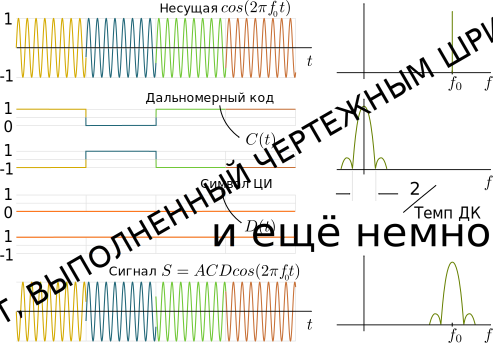
\includegraphics[keepaspectratio, width=0.8\textwidth]{inc/svg/simulation/LegacySignalsOscSpectr}
  \caption{Структура сигнала ГНСС с модуляцией дальномерным кодом и навигационным сообщением}
  \label{fig:LegacySignalsOscSpectr}
\end{figure}

В широко используемых сигналах GPS L1C/A и ГЛОНАСС L1OF в качестве спектрорасширяющей последовательности используются дальномерные коды с периодом в 1 мс и длиной 1023 и 511 символов соответственно. 
Эти последовательности являются псевдослучайными (ПСП, англ. PRN), формируются с помощью линейных генераторов на сдвиговых регистрах (англ. LFSR). 
Модель таких сигналов проста (см. рис.~\ref{fig:LegacySignalsOscSpectr}):
\begin{equation}
S\left( t  \right) = A C D \cos \left( 2 \pi f_0  t  + \varphi \right),
\end{equation}
где
\begin{itemize}
\item $A$ -- амплитуда сигнала, больше или равна нулю;
\item $C = C\left( t  \right)$ -- модуляция дальномерным кодом, принимает значения $+1$ и $-1$ при значениях дальномерного кода $0$ и $1$ соответственно, смена значений происходит часто (2 мкс или менее);
\item $D = D\left( t \right)$ -- модуляция цифровой информацией, принимает значения $+1$ и $-1$ при значениях символа цифровой информации $0$ и $1$ соответственно, смена значений происходит редко (2 мс или более);
\item $f_0$ -- несущая частота, например, 1575.42 МГц для GPS L1C/A.
\end{itemize}

\begin{figure}[ht]
  \centering
  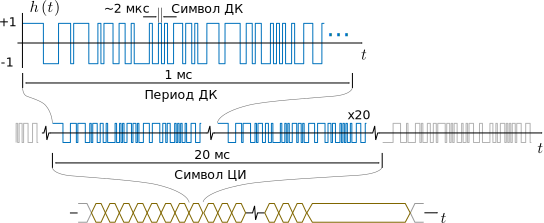
\includegraphics[keepaspectratio, width=0.8\textwidth]{inc/svg/analysis/hgraph0}
  \caption{Соотношение между темпом дальномерного кода и цифровой информации на примере сигнала ГЛОНАСС L1OF}
  \label{fig:hgraph0}
\end{figure}

Например, для всех сигналов ГЛОНАСС L1OF, принимаемых большинством современных смартфонов, используется один и тот же дальномерный код, повторяющийся каждую \textbf{миллисекунду} из года в год (см. рис.~\ref{fig:hgraph0}).

\chapter*{Послесловие} % заключение к отчёту
\renewcommand{\leftmark}{Послесловие}

Изложение итогов выполненного исследования, рекомендации, перспективы дальнейшей разработки темы

Ссылка ради ссылки \cite{perov10glonass}

\renewcommand{\leftmark}{\oldleftmark}

%%% Local Variables: 
%%% mode: latex
%%% TeX-master: "rpz"
%%% End: 
%% заключение

% % Список литературы при помощи Biber
% Юзать так:
%
% pdflatex rpz
% biber rpz
% pdflatex rpz

{
\renewcommand*{\bibfont}{\small}
\ifdefined\gostbibname \renewcommand\bibname{\gostbibname} \fi
\printbibliography
}

%%% Local Variables: 
%%% mode: latex
%%% TeX-master: "rpz"
%%% End: 


\appendix   % Тут идут приложения



\chapter{Процедуры и схемы сбора установок и стендов}
\label{cha:appendix_schemes}


Схема стенда для проверки выполнения требований назначения приведена на рис.~\ref{fig:xkcd}. 

\section{Раздел в приложении}

Перечень оборудования, задействованного в стенде на рис. \ref{fig:xkcd} приведен в табл.~\ref{tab:stend_eqip}.
	
	\begin{figure}[H]
		\centering
		\includegraphics[width=0.75\textwidth]{inc/img/appx/xkcd}
		\caption{Схема стенда прямиком с xkcd! Заодно это пример растрового рисунка}
		\label{fig:xkcd}
	\end{figure}
	
\textit{Примечание. Какое-нибудь примечание.}
	
	\begin{longtable}{|c|p{4cm}|p{11cm}|}
		\caption{Перечень оборудования, задействованного в стенде на рис. \ref{fig:xkcd}} \label{tab:stend_eqip}\\
		\hline 
		№ & Обозначение & Тип и характеристики  \\		
		\endfirsthead
		\multicolumn{3}{r}{... продолжение таблицы \ref{tab:stend_eqip}}\\ [1em] % отступ до таблицы
		\hline 
		№ & Обозначение & Тип и характеристики  \\
		\endhead
		\hline
		
		1 &  ПРМ                       & Приемник навигационных сигналов ГНСС заданных типов \\ 
		\hline 
		
		2 &  ИС  &  Имитатор навигационных сигналов, R\&S SMBV100B c не менее чем 32 каналами имитации (опции SMBVB-K136, SMBVB-K137), опциями формирования сигналов ГНСС SMBVB-K44, SMBVB-K62, SMBVB-K66, SMBVB-K94, SMBVB-K98, SMBVB-K107, опциями частотных диапазонов SMBVB-K134, SMBVB-K135.
		\\ 
		\hline 
		
		3 & Д                         & Радиочастотный сумматор-делитель мощности MiniCircuits ZAPD-2DC-S+  \\
		\hline
		
		4 & АС                         & Анализатор спектра R\&S FSV \\
		\hline
		
		5 & ИП                         & Лабораторный источник питания R\&S HAMEG HMP4040 \\
		\hline
		
		6 & ПК                         & Персональный компьютер: 
		\begin{itemize}
			\item процессор семейства Intel Core i3 и выше; 
			\item от 8 Гб оперативной памяти;
			\item наличие интерфейса Ethernet;
			\item ОС Linux Kubuntu версии от 16.04;
			\item ПО Matlab, python версии 3 и выше.
		\end{itemize} 
		\\ 
		\hline 
		
		7 & КОМ & Коммутатор (switch) Ethernet 100 Мбит/с, минимум 4 порта \\ 
		\hline 
		
		8 & -          & Кабельные сборки из состава Комплекта кабелей испытуемого образца (отмечены синим)  \\ 
		\hline 
		
		9 & -          & Дополнительные кабельные сборки и адаптеры: радиочастотных, питания, цифровых интерфейсов (отмечены красным, адаптеры могут применяться к синим) \\ 
		\hline 

		10 & -         & Табличка может быть очень длинной, с переносом на следующую страницу \\ 
		\hline 		
		
	\end{longtable}

%%% Local Variables: 
%%% mode: latex
%%% TeX-master: "rpz"
%%% End: 


\thispagestyle{empty}

\begin{center}
\textsf{Учебное издание}
\end{center}

\vspace{3cm}

\begin{center}
\textbf{Илья Владимирович Забабахин}

\vspace{10mm}

\textbf{Приемники сигналов внеземных цивилизаций\\}

\vspace{5mm}
\textbf{\small Учебное пособие для вузов}

\vspace{10mm}
Изд.№ Сдано в набор хх.хх.хх  \\
Подписано в печать хх.хх.хх \\
Формат. Бумага офсетная. \\
Гарнитура Таймс. Печать офсетная.


\vspace{10mm}
Издательство <<Радиотехника>>  \\
107031, Москва, К-31, Кузнецкий мост, д. 20/6 \\

\end{center}


\end{document}

%%% Local Variables: 
%%% mode: latex
%%% TeX-master: "rpz"
%%% End: 
